\section{Survey methodology and corpus}
\label{sec:method}

\subsection{Scope, search, and verification}

The unit of this survey is the \emph{benchmark}: an individually citeable evaluation artefact, a
suite, a dataset paired with a scoring protocol, or an interactive environment with a task
distribution, that measures robot, embodied-agent, or world-model behaviour. We deliberately exclude
three neighbouring categories that a benchmark survey is often confused with: individual models and
policies (the systems a benchmark scores), raw datasets with no scoring protocol, and pure simulators
with no task distribution. Where a work contributes both a model and a benchmark, only its benchmark
enters the corpus.

Candidates were gathered by parallel web search over arXiv, publisher venues, and project pages,
using query strings built from the cross-product of the evaluation lanes (policy, embodied,
world-model, bridge) with capability terms (manipulation, navigation, long-horizon, social,
counterfactual, physical reasoning, generation quality) and with the terms
\emph{benchmark}, \emph{evaluation}, and \emph{suite}. Every candidate was then web-verified against
its arXiv or venue page for exact title, first author, year, and identifier; any candidate that could
not be verified was dropped rather than recorded from memory, and entries were de-duplicated by both
citation key and arXiv identifier. Figure~\ref{fig:prisma} records the resulting funnel in the
PRISMA~2020 style~\cite{prisma2020}; stages that were not logged as counts are marked as such rather
than estimated. The procedure yields 160 web-verified benchmarks drawing on 164 references.

% PRISMA-2020-style corpus-construction flow with recorded counts (methodology subsection).
% Two identification streams: web-search benchmark harvest (left) and survey search (right).
% Exclusions folded inline (red italic); unlogged stages stated, never estimated.
\begin{figure}[t]
\centering
\resizebox{\textwidth}{!}{%
\begin{tikzpicture}[
  font=\footnotesize,
  box/.style={draw=hidden-draw, rounded corners=1pt, align=left, inner sep=5pt,
              text width=17em, fill=white},
  ex/.style={font=\scriptsize\itshape, text=BrickRed!85!black},
  bar/.style={draw=hidden-draw, rounded corners=1pt, inner sep=2pt, rotate=90,
              anchor=center, align=center, font=\footnotesize\bfseries, minimum width=8em},
  ar/.style={-{Stealth[length=2mm]}, darkgray, line width=0.7pt},
  node distance=4mm and 9mm,
]
% ---- left column: structured web-search benchmark stream ----
\node[box, fill=secA!30] (L1)
  {\textbf{Identification (web search).} Candidate benchmark records from five thematic sweeps
   (manipulation; navigation / driving / locomotion; long-horizon / agentic;
   world-model / video / physics; hidden-state / counterfactual / social)\\
   {\scriptsize\itshape\color{BrickRed!85!black} cross-sweep duplicates removed by name and arXiv ID; pre-dedup candidate count not logged}};
\node[box, fill=secC!22, below=of L1] (L2)
  {\textbf{Screening.} Screened against a benchmark criterion (an executable evaluation, not a dataset or model)\\
   {\scriptsize\itshape\color{BrickRed!85!black} 7 removed as datasets / models: Open X-Embodiment, DexYCB, DexGraspNet, AGIBot World, RoboCat, MimicGen, DexMimicGen}};
\node[box, fill=secC!22, below=of L2] (L3)
  {\textbf{Eligibility.} 160 metadata-verified by parallel audit agents: exact title, first author, year, arXiv ID\\
   {\scriptsize\itshape\color{BrickRed!85!black} candidates failing verification dropped at harvest (count not logged)}};
\node[box, fill=secEl, below=of L3] (L4)
  {\textbf{Landscape corpus:} 160 benchmarks (Table~\ref{tab:landscape}); 155 with an arXiv ID, 5 without};
% ---- right column: survey search ----
\node[box, fill=secB!25, right=9mm of L1] (R1)
  {\textbf{Identification (survey search).} Venue-targeted and snowball search for benchmark and
   evaluation surveys and position papers};
\node[box, fill=secB!12, below=of R1] (R2)
  {\textbf{Closest surveys:} 8 web-verified (Table~\ref{tab:survey_compare}), incl.\ one position paper};
% ---- merged included box ----
\node[box, fill=secEl, below=7mm of L4, xshift=13em, text width=35em, align=center] (INC)
  {\textbf{Included:} 160 benchmarks $+$ 8 surveys $=$ \textbf{164 references}
   (155 benchmark $+$ 8 survey $+$ 1 method; 5 benchmarks cited by name only)};
% ---- arrows ----
\draw[ar] (L1) -- (L2); \draw[ar] (L2) -- (L3); \draw[ar] (L3) -- (L4);
\draw[ar] (R1) -- (R2);
\draw[ar] (L4.south) -- (L4.south |- INC.north);
\draw[ar] (R2.south) |- ([xshift=6em]INC.north) -- ([xshift=6em]INC.north |- INC.north);
% ---- stage bars ----
\node[bar, fill=secA] at ($(L1.west)+(-2em,0)$) {Identification};
\node[bar, fill=secC] at ($(L2.west)!0.5!(L3.west)+(-2em,0)$) {Screening};
\node[bar, fill=secE] at ($(L4.west)+(-2em,0)$) {Included};
\end{tikzpicture}}
\caption{\textbf{Corpus construction} in the PRISMA 2020 style~\citep{prisma2020}. The left column is
the web-search stream behind the landscape corpus (Table~\ref{tab:landscape}): five thematic sweeps,
de-duplicated by name and arXiv ID, screened to drop datasets and models, and metadata-verified by
parallel audit agents. The right column is the venue-targeted and snowball search behind the closest
surveys (Table~\ref{tab:survey_compare}). Both streams feed the included set. Candidates whose
metadata could not be verified were discarded at harvest; their count was not logged, which we state
rather than estimate.}
\Description{A PRISMA 2020 style flow diagram with two identification columns. The left column
(structured web search) shows candidate benchmark records from five thematic sweeps, de-duplicated by
name and arXiv ID, screened to remove seven datasets and models, and 160 metadata-verified records
forming the landscape corpus (155 with an arXiv ID, 5 without). The right column (survey search)
yields 8 closest surveys including one position paper. Both columns feed an included box of 160
benchmarks plus 8 surveys and one methodology citation, totalling 164 references.}
\label{fig:prisma}
\end{figure}


\subsection{Placement, definitions, and the core-versus-appendix rule}

Each benchmark is placed on four axes: its evaluation \emph{lane} (Section~\ref{sec:taxonomy}), the
robotic \emph{capability} it primarily stresses, its evaluation \emph{mode} (open-loop prediction or
generation quality, closed-loop task success, or a prediction-to-action bridge), and whether it
builds a native VLA-versus-world-model \emph{contrast} (explicit, partial, or model-agnostic).
Table~\ref{tab:defs} states the operational definition used for each placement, so that boundary
cases are resolved by a written rule rather than by taste; a benchmark counts as building a contrast,
for example, only if a direct-policy and a world-model policy are run under one protocol and compared.

Because the full corpus is large, we split it. A benchmark enters the core taxonomy
(Figure~\ref{fig:taxonomy_main}) when it is cleanly axis-placeable, distinct from its neighbours, and
fully characterisable from its paper; the 86 representative benchmarks that meet all three sit in the
taxonomy, and the complete set of 160 is catalogued in the landscape table
(Table~\ref{tab:landscape}, Appendix~\ref{app:landscape}). Every count in the survey reconciles with
that table.

% Table 3 -- operational definitions of the evaluation modes and the two contrast tests.
% These resolve the boundary cases a benchmark survey must adjudicate (mirrors P1 Table 3).
\begin{table*}[t]
\centering
\footnotesize
\setlength{\tabcolsep}{5pt}
\renewcommand{\arraystretch}{1.3}
\resizebox{\textwidth}{!}{%
\begin{tabular}{@{}p{0.19\textwidth} p{0.40\textwidth} p{0.30\textwidth}@{}}
\toprule
\textbf{Construct} & \textbf{Counts (a benchmark has it if and only if\ldots)} & \textbf{Does not count} \\
\midrule
\textbf{Open-loop eval (\dopen)} &
it scores prediction or generation \emph{quality} on fixed inputs without executing the
prediction in a feedback loop: video fidelity (FVD), physics or rollout consistency, or
frame-level accuracy &
any protocol where an action is executed and the environment responds; offline scoring of a
policy's success \\
\textbf{Closed-loop eval (\dclosed)} &
success is measured by running a policy \emph{in} the environment with state feedback and
scoring task outcome: success rate, sub-goal completion, or reward under interaction &
scoring a generated video or a static prediction; a metric computed without stepping the
environment \\
\textbf{Bridge (\dbridge)} &
a prediction (imagined rollout, video, or latent plan) is \emph{converted into executed actions}
and scored on the resulting task success &
a benchmark that stops at prediction quality; one that never turns a prediction into a control
signal \\
\textbf{Native VLA-vs-WM contrast ($\gamma$)} &
the benchmark \emph{itself} runs both a direct Vision-Language-Action policy and a world-model
policy under one protocol and reports the head-to-head &
a model-agnostic suite that merely \emph{hosts} either family; a suite evaluated with only one
family in the original paper \\
\textbf{Advantage-of-prediction ($\delta$)} &
a metric quantifies the closed-loop \emph{gain} of a predictive policy over a matched direct-VLA
baseline on the same tasks (assessed, not adopted) &
absolute success with no matched baseline; open-loop quality scores; a ranking that never
isolates the predictive component \\
\bottomrule
\end{tabular}}
\caption{Operational definitions used to place each benchmark on the evaluation axes
(\S\ref{sec:method}). They resolve the ambiguous boundary cases: hosting a policy is not the same
as \emph{building} a VLA-vs-world-model contrast ($\gamma$), and an absolute success number is not
an advantage-of-prediction measurement ($\delta$) without a matched baseline. \dopen\ open-loop,
\dclosed\ closed-loop, \dbridge\ bridge.}
\label{tab:defs}
\end{table*}


\subsection{The corpus at a glance}

Figures~\ref{fig:corpus_overview} and~\ref{fig:corpus_dist} profile the corpus, with all counts
re-tallied directly from the catalogue rather than taken from any single paper. The 160 benchmarks
divide by lane into 37 policy suites, 85 embodied-agent benchmarks, 34 world-model-evaluation
benchmarks, and 4 prediction-to-action bridges, and by capability area into twelve clusters led by
long-horizon planning (26), manipulation and dexterity (22), and generation quality (19). By
evaluation mode, 113 score closed-loop task success, 43 score open-loop prediction or generation, and
only 4 bridge the two. Publication years show the field's shape clearly: a steady rise from 2 in 2017
to a peak of 36 in 2024, with the world-model-evaluation lane arriving almost entirely in the last
three years (Figure~\ref{fig:lane_trend}). The single most consequential distribution is the contrast
axis: 138 of 160 benchmarks are model-agnostic, 11 build a partial contrast, and 11 (7\%) build one
explicitly. That imbalance is the empirical core of the survey and is taken up in
Section~\ref{sec:gap}.

% Survey-at-a-glance overview. Every number is real: 160 benchmarks, 164 references, 4 lanes,
% 2017-2026 span, 11 explicit contrasts. Per-area bars are kindred capability clusters merged
% (dexterous into manipulation, VLN into navigation, ToM into hidden-state); the 12 areas sum to 160.
\begin{figure}[tp]
\centering
\resizebox{\textwidth}{!}{%
\begin{tikzpicture}
% ---- stat callouts ----
\foreach [count=\i] \num/\lab in {160/benchmarks, 164/references, 4/{eval.\ lanes},
                                  12/{capability areas}, 11/{explicit contrasts}, {2017--26}/span}{
  \node[draw=hidden-draw, rounded corners=2pt, fill=secA!14, minimum width=1.9cm,
        minimum height=1.15cm, align=center] at ({\i*2.05-0.2},4.9)
        {{\large\bfseries\num}\\[1pt]{\scriptsize\lab}};
}
% ---- per-capability-area horizontal bar chart ----
\foreach [count=\i] \l/\v/\c in {{Long-horizon \& planning}/26/cat-code,
   {Manipulation \& dexterity}/22/cat-vla, {Generation quality}/19/cat-skill,
   {Navigation (incl.\ VLN)}/16/cat-code, {Physical reasoning}/13/cat-skill,
   {Social \& multi-agent}/12/cat-code, {Hidden-state \& ToM}/9/cat-code,
   {Counterfactual}/9/cat-skill, {Autonomous driving}/9/cat-code,
   {Generalization}/7/cat-vla, {Locomotion}/6/cat-code, {Other areas}/12/gray}{
  \fill[\c!70!black] (4.4,{3.75-\i*0.315}) rectangle ({4.4+\v*0.235},{3.75-\i*0.315+0.24});
  \node[left=2pt,font=\scriptsize] at (4.4,{3.75-\i*0.315+0.12}) {\l};
  \node[right=1.5pt,font=\scriptsize] at ({4.4+\v*0.235},{3.75-\i*0.315+0.12}) {\v};
}
\node[font=\footnotesize\bfseries] at (7.3,3.95) {Benchmarks per capability area (160 total)};
\end{tikzpicture}}
\caption{\textbf{The catalogued corpus at a glance.} The survey maps 160 web-verified benchmarks
across 4 evaluation lanes, spanning 2017--2026 and totalling 164 references; only 11 build an
explicit Vision-Language-Action vs world-model contrast. The bars give benchmarks per capability
area, with kindred clusters merged (dexterity into manipulation, vision-language navigation into
navigation, theory-of-mind into hidden-state); the twelve areas sum to the 160 works of
Table~\ref{tab:landscape}. Bars are coloured by the dominant lane of each area (teal policy, blue
embodied, purple world-model).}
\Description{An overview figure. Six stat callouts read: 160 benchmarks, 164 references, 4
evaluation lanes, 12 capability areas, 11 explicit contrasts, span 2017 to 2026. Below, a horizontal bar chart gives
benchmarks per capability area: long-horizon and planning 26, manipulation and dexterity 22,
generation quality 19, navigation 16, physical reasoning 13, social and multi-agent 12, hidden-state
and theory-of-mind 9, counterfactual 9, autonomous driving 9, generalization 7, locomotion 6, other
areas 12.}
\label{fig:corpus_overview}
\end{figure}

% Corpus distribution charts. Bar heights are the REAL tallies of the 160 catalogue benchmarks
% (year, lane, eval mode, VLA-vs-WM contrast), re-counted from docs/assets/catalog_p3.js.
\begin{figure*}[tp]
\centering
\definecolor{pal1}{HTML}{C0392B}\definecolor{pal2}{HTML}{E67E22}\definecolor{pal3}{HTML}{B7950B}%
\definecolor{pal4}{HTML}{1E8449}\definecolor{pal5}{HTML}{7D3C98}\definecolor{pal6}{HTML}{C2185B}%
\definecolor{pal7}{HTML}{566573}\definecolor{pal8}{HTML}{6E2C00}\definecolor{pal9}{HTML}{7B241C}%
\definecolor{pal10}{HTML}{4A235A}%
\resizebox{\textwidth}{!}{%
\begin{tabular}{@{}c@{\hspace{7mm}}c@{}}
% ---- (a) benchmarks per year ----
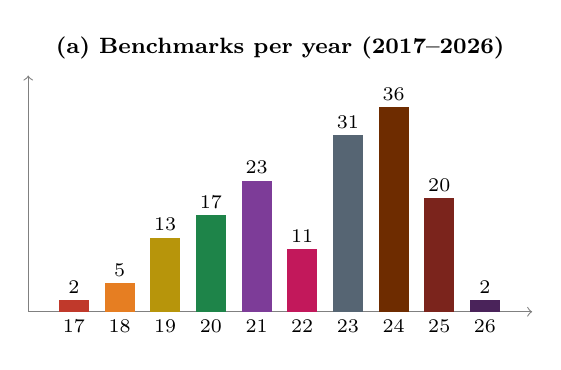
\begin{tikzpicture}[baseline]
  \draw[->,gray] (0,0)--(0,3.0); \draw[->,gray] (0,0)--(6.4,0);
  \foreach [count=\i] \l/\v in {17/2,18/5,19/13,20/17,21/23,22/11,23/31,24/36,25/20,26/2}{
    \fill[pal\i] ({\i*0.58-0.19},0) rectangle ({\i*0.58+0.19},{\v*0.0722});
    \node[font=\scriptsize] at ({\i*0.58},-0.18) {\l};
    \node[font=\scriptsize,above=-1pt] at ({\i*0.58},{\v*0.0722}) {\v};
  }
  \node[font=\footnotesize\bfseries] at (3.2,3.35) {(a) Benchmarks per year (2017--2026)};
\end{tikzpicture}
&
% ---- (b) evaluation lane ----
\begin{tikzpicture}[baseline]
  \draw[->,gray] (0,0)--(0,3.0); \draw[->,gray] (0,0)--(5.0,0);
  \foreach [count=\i] \l/\v/\c in {policy/37/cat-vla, embodied/85/cat-code,
                                    {wm-eval}/34/cat-skill, bridge/4/cat-bench}{
    \fill[\c!75!black] ({\i*1.1-0.3},0) rectangle ({\i*1.1+0.3},{\v*0.0306});
    \node[font=\scriptsize] at ({\i*1.1},-0.18) {\l};
    \node[font=\scriptsize,above=-1pt] at ({\i*1.1},{\v*0.0306}) {\v};
  }
  \node[font=\footnotesize\bfseries] at (2.5,3.35) {(b) Evaluation lane};
\end{tikzpicture}
\\[7mm]
% ---- (c) evaluation mode (horizontal) ----
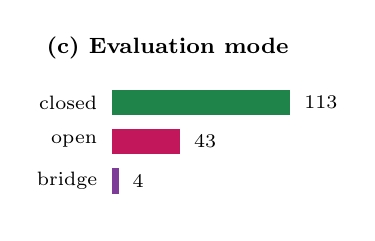
\begin{tikzpicture}[baseline]
  \foreach [count=\i] \l/\v/\c in {closed/113/pal4, open/43/pal6, bridge/4/pal5}{
    \fill[\c] (1.5,{1.75-\i*0.5}) rectangle ({1.5+\v*0.020},{1.75-\i*0.5+0.32});
    \node[left=2pt,font=\scriptsize] at (1.5,{1.75-\i*0.5+0.16}) {\l};
    \node[right=1.5pt,font=\scriptsize] at ({1.5+\v*0.020},{1.75-\i*0.5+0.16}) {\v};
  }
  \node[font=\footnotesize\bfseries] at (2.2,2.1) {(c) Evaluation mode};
\end{tikzpicture}
&
% ---- (d) VLA-vs-WM contrast (horizontal; the thesis panel) ----
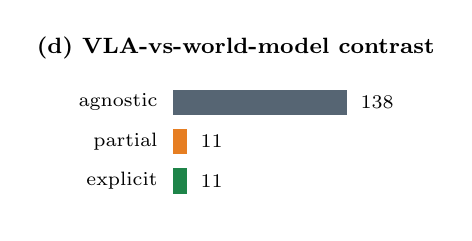
\begin{tikzpicture}[baseline]
  \foreach [count=\i] \l/\v/\c in {agnostic/138/pal7, partial/11/pal2, explicit/11/pal4}{
    \fill[\c] (1.6,{1.75-\i*0.5}) rectangle ({1.6+\v*0.016},{1.75-\i*0.5+0.32});
    \node[left=2pt,font=\scriptsize] at (1.6,{1.75-\i*0.5+0.16}) {\l};
    \node[right=1.5pt,font=\scriptsize] at ({1.6+\v*0.016},{1.75-\i*0.5+0.16}) {\v};
  }
  \node[font=\footnotesize\bfseries] at (2.4,2.1) {(d) VLA-vs-world-model contrast};
\end{tikzpicture}
\end{tabular}}
\caption{\textbf{Profile of the 160 catalogue benchmarks} (Table~\ref{tab:landscape}), re-counted
directly from the catalogue. (a)~publication year, showing the 2023--2024 surge; (b)~evaluation lane
(embodied navigation dominates, then policy suites); (c)~evaluation mode (closed-loop task success
dominates, open-loop prediction is second, only four bridges reach action); (d)~whether the benchmark
builds a native Vision-Language-Action vs world-model contrast, the survey's organising question:
\textbf{138 of 160 are model-agnostic}, and only \textbf{11 (7\%)} build the contrast explicitly.
Counts are the exact column tallies of Table~\ref{tab:landscape}.}
\Description{Four bar charts of the 160 benchmarks. (a) Benchmarks per year rise from 2 in 2017 to 31
in 2023 and 36 in 2024, then 20 in 2025. (b) Evaluation lane: policy 37, embodied 85, world-model
evaluation 34, bridge 4. (c) Evaluation mode: closed 113, open 43, bridge 4. (d) VLA-vs-world-model
contrast: model-agnostic 138, partial 11, explicit 11, with a note that only 11 (7 percent) build a
contrast.}
\label{fig:corpus_dist}
\end{figure*}

% Real per-year counts of closed-loop vs open-loop benchmarks (year x eval tally from catalog_p3.js).
% The story: open-loop world-model evaluation surges and overtakes closed-loop in 2025.
\begin{figure}[t]
\centering
\definecolor{cclosed}{HTML}{1E8449}\definecolor{copen}{HTML}{C2185B}%
\resizebox{\textwidth}{!}{%
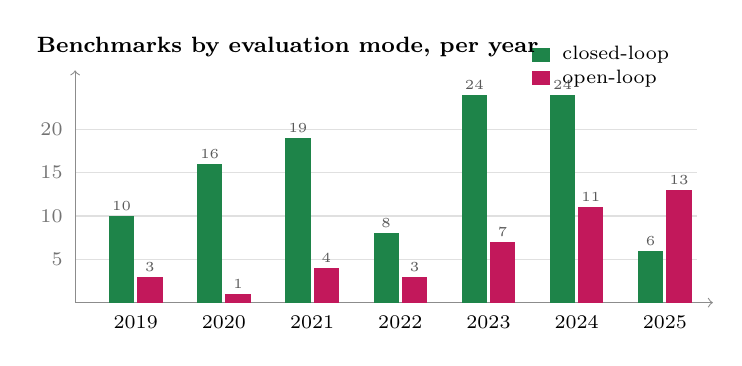
\begin{tikzpicture}
  \foreach \i in {5,10,15,20}{\node[font=\scriptsize,left=1pt,text=black!55] at (0.5,{\i*0.11}) {\i};
    \draw[black!12] (0.5,{\i*0.11})--(8.4,{\i*0.11});}
  \draw[->,black!45] (0.5,0)--(0.5,2.95); \draw[->,black!45] (0.5,0)--(8.6,0);
  \foreach [count=\g] \yr/\c/\o in {2019/10/3,2020/16/1,2021/19/4,2022/8/3,2023/24/7,2024/24/11,2025/6/13}{
    \pgfmathsetmacro\x{\g*1.12+0.15}
    \fill[cclosed] ({\x-0.34},0) rectangle ({\x-0.02},{\c*0.11});
    \fill[copen]   ({\x+0.02},0) rectangle ({\x+0.34},{\o*0.11});
    \node[font=\tiny,text=black!65,above=-1.5pt] at ({\x-0.18},{\c*0.11}) {\c};
    \node[font=\tiny,text=black!65,above=-1.5pt] at ({\x+0.18},{\o*0.11}) {\o};
    \node[font=\scriptsize] at (\x,-0.25) {\yr};}
  % legend (top-right, 2-row, above the value labels so it clears the tall centre bars; matches p1_fig7)
  \fill[cclosed] (6.3,3.06) rectangle (6.53,3.24);
  \node[font=\scriptsize,right=1pt] at (6.53,3.15) {closed-loop};
  \fill[copen] (6.3,2.76) rectangle (6.53,2.94);
  \node[font=\scriptsize,right=1pt] at (6.53,2.85) {open-loop};
  \node[font=\footnotesize\bfseries] at (3.2,3.25) {Benchmarks by evaluation mode, per year};
\end{tikzpicture}}
\caption{\textbf{The world-model-evaluation wave is recent.} Per-year counts of closed-loop
task-success benchmarks (green) and open-loop world-model / video-generation benchmarks (magenta) in
the catalogue. Closed-loop suites dominate through 2024; in \textbf{2025 open-loop evaluation
overtakes them} (13 vs 6) as the world-model-generation literature arrives. The four
prediction-to-action bridges are newer still, all appearing in 2024 or later. Years are the
benchmarks' first-release years (2026 is partial and omitted); counts are the tallies of
Table~\ref{tab:landscape}.}
\Description{A grouped bar chart of benchmarks by evaluation mode per year, 2019 to 2025. Closed-loop
(green): 10, 16, 19, 8, 24, 24, 6. Open-loop (magenta): 3, 1, 4, 3, 7, 11, 13. Closed-loop dominates
until 2024, then open-loop overtakes it in 2025.}
\label{fig:lane_trend}
\end{figure}

